\section{Introduction}



Current neural networks are expected to generalize to unseen distributions in real-world applications, which can break the independent
and identically distributional (I.I.D.) assumption of traditional machine learning algorithms \cite{zhou2021domain,wang2022generalizing}. The distribution shift between training and test data may largely deteriorate most current approaches in practice. Hence, instead of generalization within the training distribution, the ability to generalize under distribution shift, namely domain generalization (DG) \cite{muandet2013domain}, has attracted increasing attention \cite{wang2022generalizing}.

Various methods have been proposed to address the DG problem recently, many of which have shown promising performance. As a learning problem mainly in the computer vision field, the DG task relies highly on the chosen optimizer, yet the effect of the optimizer in DG has hardly been studied. Most current algorithms, following the well-known benchmark DomainBed \cite{gulrajani2020search}, default to optimize models with Adam \cite{kingma2014adam} without considering other optimizers. 
However, the in-distribution generalization ability of popular optimizers has been investigated from the perspective of loss landscape recently \cite{foret2021sharpness,gan2020large} and Adam is found to achieve inferior generalization compared with other optimizers such as SGD \cite{nesterov1983method} due to the sharp minima Adam selected. Thus, investigating the impact of optimizers in DG and clarifying whether Adam should be considered as the default optimizer is of significance. 

\begin{figure}[t]
    \centering
    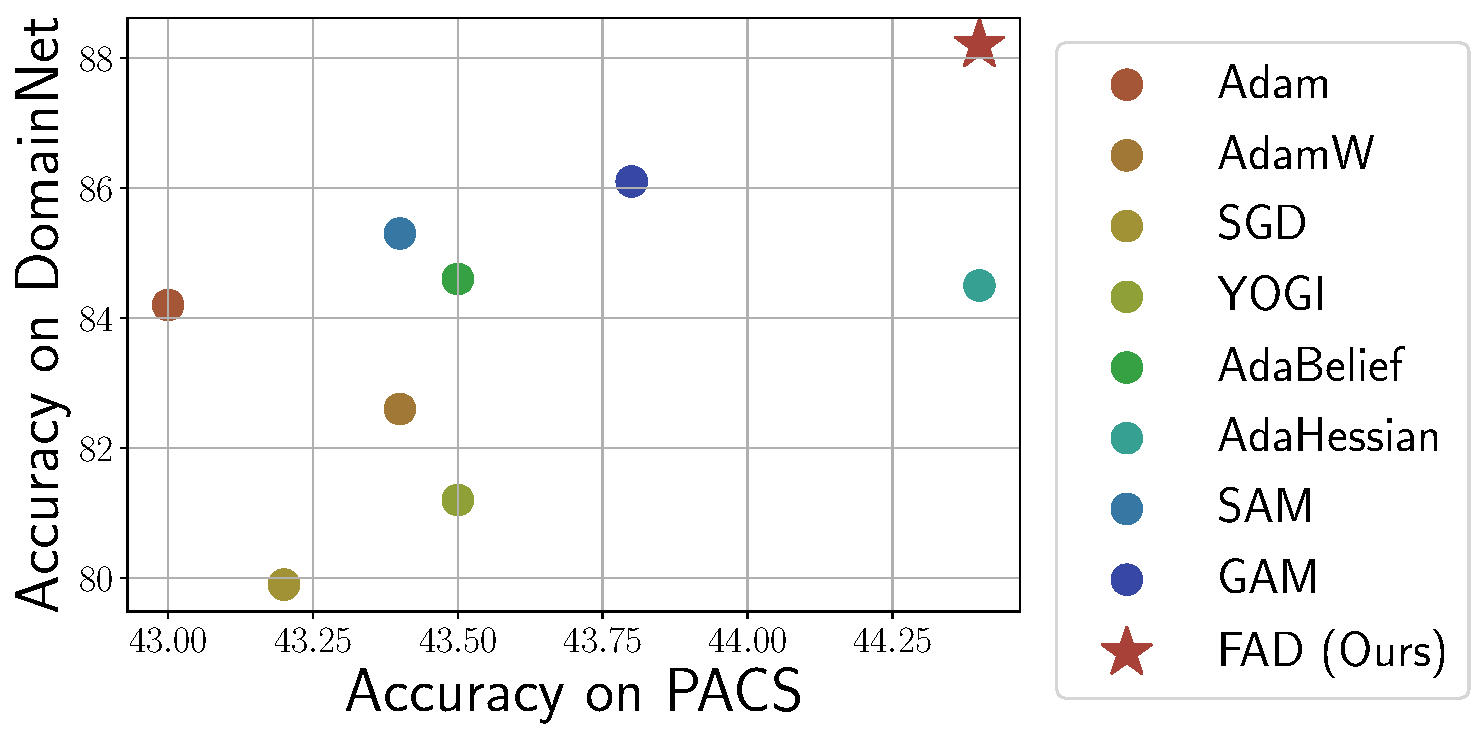
\includegraphics[width=\linewidth]{figs/acc_pacs_domainnet.pdf}
    \caption{Test accuracy on PACS and DomainNet of different optimizers. Adam, the default optimizer in popular benchmarks shows no advantage compared with its counterparts, while the proposed FAD achieve better OOD generalization performance compared with current optimizers.}
    \label{fig:intro-pacs-domainnet}
\end{figure}

In this paper, we empirically compare the performance of current optimizers, including Adam, SGD, AdaBelief \cite{zhuang2020adabelief}, YOGI \cite{zaheer2018adaptive}, AdaHessian \cite{yao2021adahessian}, SAM \cite{foret2021sharpness}, and GAM\cite{Zhang2023GradientNA}.  
Through extensive experiments on current DG benchmarks, we show that Adam can hardly surpass other optimizers on most DG datasets. The best choice of the optimizer for different DG methods varies across different datasets, and choosing the right optimizer can help exceed the current leaderboards' limitations. 

Recently, the connection between the flatness of the loss landscape and in-distribution generalization ability has been widely studied and verified both theoretically\cite{zhuang2022surrogate} and empirically\cite{du2022sharpness}.  
Some works \cite{cha2021swad, rangwani2022closer} show that flatness also leads to superior OOD generalization. However, none of the previous works consider the optimization in DG nor provide theoretical assurance of their approach. 
Among flatness-aware optimization methods, sharpness-Aware Minimization (SAM) \cite{foret2021sharpness} and its variants \cite{zhuang2022surrogate, kwon2021asam,zhong2022improving,kim2022sharpness}, which optimize the zeroth-order flatness, achieve SOTA performance on various in-distribution image classification tasks \cite{kwon2021asam,zhuang2022surrogate}. Most recently, Gradient Norm Aware Minimization (GAM) \cite{Zhang2023GradientNA} shows that minimizing the first-order flatness provides a more substantial penalty on the sharpness of minima than zeroth-order flatness yet requires more computation overhead. 
Due to the first-order Taylor expansions adopted to optimize zeroth-order and first-order flatness, both SAM and GAM lose some of their penalty strength, and thus they can be mutually reinforced by each other. To accelerate the optimization of first-order flatness and combine zero-order flatness, we propose a unified optimization framework, Flatness-Aware minimization for Domain generalization (FAD), which eliminates the considerable computation overhead for Hessian or Hessian-vector products. 
We theoretically show that the proposed FAD controls the dominant eigenvalue of Hessian of the training loss, which indicates the sharpness of the loss landscape along its most critical direction \cite{kaur2022maximum}.
We present an OOD generalization bound to show that the proposed FAD guarantees the generalization error on test data and convergence analysis. Through extensive experiments, we evaluate FAD and other optimizers on various DG benchmarks. 



We summarize the main contribution as follows.
\begin{itemize}[noitemsep,topsep=0pt,parsep=0pt,partopsep=0pt]
    \item We propose a unified optimization framework, Flatness-Aware minimization for Domain generalization (FAD), to optimize zeroth-order and first-order flatness simultaneously. Without calculating Hessian and Hessian-vector products, FAD considerably reduces the computation overhead of first-order flatness.
    \item We theoretically analyze the OOD generalization error and convergence of FAD. We show that FAD controls the dominant eigenvalue of Hessian and thus the flatness of learned minima.
    \item We empirically show that Adam, the default optimizer for most current DG benchmarks, can hardly be the optimal choice for most DG datasets. We present the superiority of FAD compared with current optimizers through extensive experiments.
    \item We empirically validate that FAD finds flatter optima with lower Hessian spectra compared with zeroth-order and first-order flatness-aware optimization methods.
\end{itemize}







 